\documentclass{article}
\usepackage{tikz}

\begin{document}

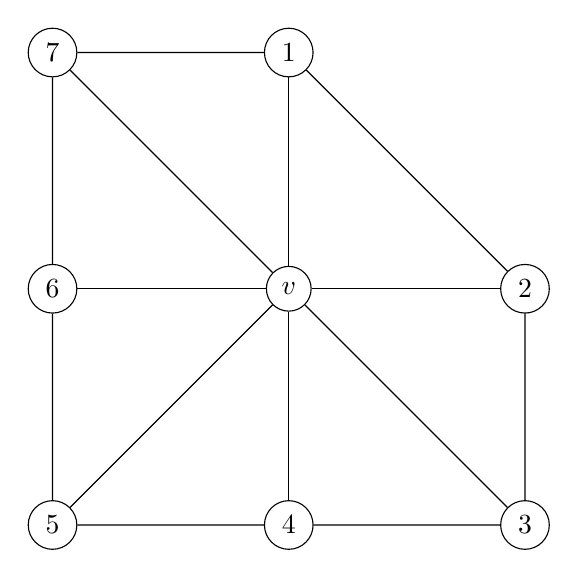
\begin{tikzpicture}[scale=1.5]
    % Define nodes
    \node (1) at (0,2) [circle,draw] {1};
    \node (2) at (2,0) [circle,draw] {2};
    \node (3) at (2,-2) [circle,draw] {3};
    \node (4) at (0,-2) [circle,draw] {4};
    \node (5) at (-2,-2) [circle,draw] {5};
    \node (6) at (-2,0) [circle,draw] {6};
    \node (7) at (-2,2) [circle,draw] {7};
    \node (v) at (0,0) [circle,draw] {$v$};

    % Draw edges
    \draw (1) -- (2);
    \draw (2) -- (3);
    \draw (3) -- (4);
    \draw (4) -- (5);
    \draw (5) -- (6);
    \draw (6) -- (7);
    \draw (7) -- (1);
    \draw (1) -- (v);
    \draw (2) -- (v);
    \draw (3) -- (v);
    \draw (4) -- (v);
    \draw (5) -- (v);
    \draw (6) -- (v);
    \draw (7) -- (v);
\end{tikzpicture}

\end{document}